\documentclass[letterpaper,12pt]{article}
\usepackage{array}
\usepackage{threeparttable}
\usepackage{geometry}

\usepackage{natbib}

%\usepackage{jf} %always check the instruction of the package to see if it conflicts
\geometry{letterpaper,tmargin=1in,bmargin=1in,lmargin=1.25in,rmargin=1.25in}
\usepackage{fancyhdr,lastpage}
\pagestyle{fancy}
\lhead{}
\chead{}
\rhead{}
\lfoot{}
\cfoot{}
\rfoot{\footnotesize\textsl{Page \thepage\ of \pageref{LastPage}}}
\renewcommand\headrulewidth{0pt}
\renewcommand\footrulewidth{0pt}
\usepackage[format=hang,font=normalsize,labelfont=bf]{caption}
\usepackage{listings}
\lstset{frame=single,
  language=Python,
  showstringspaces=false,
  columns=flexible,
  basicstyle={\small\ttfamily},
  numbers=none,
  breaklines=true,
  breakatwhitespace=true
  tabsize=3
}
\usepackage{amsmath}
\usepackage{amssymb}
\usepackage{amsthm}
%\usepackage{harvard}
\usepackage{setspace}
\usepackage{float,color}
\usepackage[pdftex]{graphicx}
\usepackage{hyperref}
\hypersetup{colorlinks,linkcolor=red,urlcolor=blue,citecolor=blue}
\theoremstyle{definition}
\newtheorem{theorem}{Theorem}
\newtheorem{acknowledgement}[theorem]{Acknowledgement}
\newtheorem{algorithm}[theorem]{Algorithm}
\newtheorem{axiom}[theorem]{Axiom}
\newtheorem{case}[theorem]{Case}
\newtheorem{claim}[theorem]{Claim}
\newtheorem{conclusion}[theorem]{Conclusion}
\newtheorem{condition}[theorem]{Condition}
\newtheorem{conjecture}[theorem]{Conjecture}
\newtheorem{corollary}[theorem]{Corollary}
\newtheorem{criterion}[theorem]{Criterion}
\newtheorem{definition}[theorem]{Definition}
\newtheorem{derivation}{Derivation} % Number derivations on their own
\newtheorem{example}[theorem]{Example}
\newtheorem{exercise}[theorem]{Exercise}
\newtheorem{lemma}[theorem]{Lemma}
\newtheorem{notation}[theorem]{Notation}
\newtheorem{problem}[theorem]{Problem}
\newtheorem{proposition}{Proposition} % Number propositions on their own
\newtheorem{remark}[theorem]{Remark}
\newtheorem{solution}[theorem]{Solution}
\newtheorem{summary}[theorem]{Summary}
%\numberwithin{equation}{section}
%\bibliographystyle{aer}
\newcommand\ve{\varepsilon}
\newcommand\boldline{\arrayrulewidth{1pt}\hline}

\DeclareMathOperator*{\argmax}{arg\,max}

\usepackage{graphicx}
\graphicspath{ {c:/users/yafei/compecon_fall17/visualization} }

\title{Problem Set 5: Visualization}
\author{Yafei Zhang \thanks{Yafei Zhang is from Finance department of USC, he can be reached at yafei.zhang@grad.moore.sc.edu.}}
\date{October 17 2017}

\begin{document}

\maketitle

\vspace{5mm}

\section{Intuition}

I am interested in analyzing private placement, a very commonly used channel to raise external financing especially for private firms, in United States. Specifically, I concentrate on the impact of National Securities Markets Improvement Act of 1996 (here and after NSMIA) on the frequency and amount of private placements conducted by private firms in U.S.. This Act is documented by a lot of law reviewers to be very important to the capital market in U.S., especially for the private placement industry.

Prior to 1996, private placement is exempted from the federal regulation according to the 1934 Securities Act. However, it is under supervision of state governments, i.e., the so-called Blue Sky Laws. Different states have very different restrictions and exemptions on private placements. For example, some states require the number of institutional buyers to be less than 15 but some others may allow more or less buyers \cite{royalty1976private}. After 1996 when NSMIA was implemented, state governments did not have authority to regulate the private placement any more. They could intervene only when the issuer misbehaved and hurt the investors. As such, I suspect that this Act further relaxed the regulation on private placements \cite{johnson2010private}, which would increase the use of private placement for external finance.


\section{Data introduction}

The data used for the three figures in this problem set is downloaded from S\&P Capital IQ database. I collect private placements of U.S. private firms from 1985 to 2006. The original sample consists of around 26,000 observations. The variables of my interest are year, state of the issuer, the amount of the private placement, and the round of the private placement \footnote{A firm might sell their shares privately for multiple times. And it is usually categorized into rounds 1, 2, and 3, etc. Some firms can raise private funds for more than ten rounds.}.

Before I plot any figures, I exclude private placements with zero or missing values. I apply specific filters to the data when I draw Figures 2 and 3. For example, to plot Figure 2, I only keep the first three round of private placements. For Figure 3, I drop observations with missing states.

\section{Figure interpretation}

\subsection{Figure 1}

In this subsection, I present the results of Figure \ref{fig:figure1}. It plots the aggregated number and value of private placements across years (from 1985 to 2006) for all the U.S. private firms. That is, the amount and number in the figure are aggregated value for each year.

\begin{figure}[h]
	\centering
	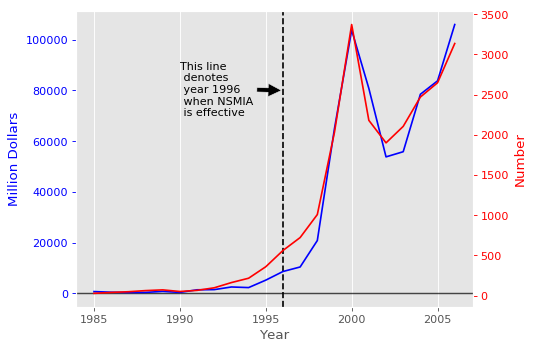
\includegraphics[width=\textwidth]{figure1}
	\caption{Number and Amount of Private Placement across Years}
	\label{fig:figure1}
\end{figure}

The x axis denotes the year. The left y axis which is colored by blue is the amount of private placements in million dollars. And the right y axis which is colored by red is the number of private placements. Accordingly, the blue line in the figure represents the time trend of amount while the red line refers to the time trend of the number. I add a vertical line which is dotted with black for year 1996 to indicate that this line denotes the year when NSMIA is implemented by the federal government.

The figure shows that before 1994, both number and amount of private placements were very low and did not vary too much. Then they started to increase dramatically, especially after 1998. They both reached their peaks at 2000 and experienced a sharp decline after that for two years. Then they got back the increasing trend and kept soaring until the end of this sample period. This suggests that it is not very convincing, at least based on this single picture, to view NSMIA as a cutpoint year because the increase starts from two years prior to 1996. To get more sense on the potential impacts of NSMIA in 1996, more visualizations are needed.

\subsection{Figure 2}

This subsection shows the results of Figure \ref{fig:figure2}. This figure plots the number of private placements for rounds 1, 2, and 3 across years \footnote{I only select rounds 1, 2, and 3 for the analysis in this section. Because most firms issue less than three rounds in terms of private placements although there are some firms issue more than ten rounds. Another reason is that if NSMIA can facilitate the private issuance, I would expect that many firms who have not conducted private placement ever would more likely to take advantage of it if the benefits dominate the costs.}.

\begin{figure}[h]
	\centering
	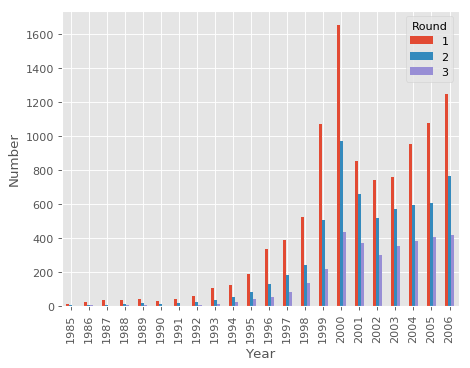
\includegraphics[width=\textwidth]{figure2}
	\caption{Number and Amount of Private Placement for Different Rounds across Years}
	\label{fig:figure2}
\end{figure}

The x axis indicates the year, the y axis is the number. In the figure, there are three bars colored with different rounds and clustered together for each year. Red, Blue, and Purple refers to round 1, 2, and 3, respectively (Please also see the legend in the top-right corner).

This figure shows a very similar pattern as Figure \ref{fig:figure1}. Particularly, it suggests that most firms issue private placement once. And there is probably a negative monotonic relationship between number of issuers and the round number. I.e., larger the round number, fewer issuers. Besides, the numbers for all the rounds were very low and did not change much before 1992. But they increased exponentially from 1993 to 2000 when the peaks were reached. Then they experienced a sharp drop for two years until 2002 from when they started to increase again.

The conclusion from this picture is the same as Figure \ref{fig:figure1}. Namely, the impact of NSMIA is not obvious since the pattern or trend starts earlier than the year that NSMIA is effective.


\subsection{Figure 3}

This subsection reports a figure regarding number of private placements across states in U.S.. The number of private placement is an aggregated value across years for each states. The color bar below the figure denotes the relationship between the darkness of the color and the log value of number of private placements. If the color of a state in the map is more toward to the right of the color bar, the number of private placement in that state is higher.

\begin{figure}[h]
	\centering
	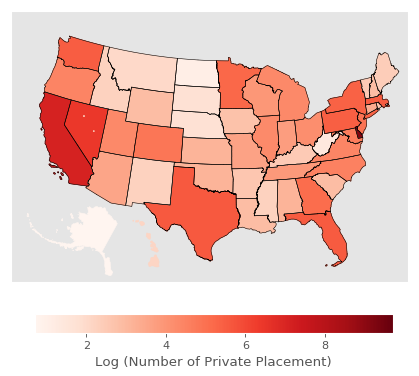
\includegraphics[width=\textwidth]{figure3}
	\caption{Private Placement across States in U.S.}
	\label{fig:figure3}
\end{figure}

The figure demonstrates that the activeness of private placement varies across states. Firms located in the West and East are more likely to raise money via private placement, while firms in the Middle are relatively inactive. California and Delaware enjoy the higher frequency of private placements for the private firms there. Other states such as Texas, Florida, Georgia, New York, Nevada, Pennsylvania, Minnesota do not issue private placement as frequent as California and Delaware, but they have number of private placement above 403 ($ e^{6} $). Most of the rest states have around 55 ($ e^{4} $) private placements on average, which is relatively low.

The reason for me to draw this map is to get a sense of the private placements across states. Since I don't find significant pattern change before and after NSMIA, I would suspect that the effect of NSMIA might be different across states given the important role played by this Act in U.S. capital market. To deepen the analysis with respect to this topic, I would try to find variation across states of implementing NSMIA. Then, I would be able to disentangle the impacts and gauge the economic effects of this Act.

\clearpage
\bibliographystyle{apalike}
\bibliography{PS5_library}

\end{document}